\documentclass[a4paper, 11pt]{article}
\usepackage[left=3cm, top=3cm, right=2cm, bottom=2cm]{geometry}
%pacote que define as margens
\usepackage{helvet}\renewcommand{\familydefault}{\sfdefault} % define a fonte ARIAL como padrão do texto
\usepackage[utf8]{inputenc} %pacote que permite a utilização de acentos
\usepackage[T1]{fontenc}
\usepackage[brazil]{babel} %pacote que define o idioma
\usepackage{graphicx} %pacote que permite a inserção de imagens
\pagestyle{myheadings} %pacote que define o cabeçalho com o número de página no canto superior direito
\usepackage{setspace} %pacote que permite especificar o espaçamento entre linhas no documento
\usepackage{indentfirst}\setlength{\parindent}{1cm} %pacote que faz indentação na primeira linha do parágrafo
\usepackage{float} %Pacote que permite tabelas flutuarem em qualquer posição
\usepackage[alf,abnt-repeated-title-omit=yes,abnt-emphasize=bf,abnt-etal-list=0]{abntex2cite} %define os parâmetros necessários para as referências e citações de acordo com a ABNT
\usepackage{amsthm} % Pacote que permite a utilização de teoremas
\usepackage{amsfonts} % Pacote que permite a utilização de símbolos matemáticos
\usepackage{caption} % Pacote que permite a inserção de legendas em figuras
\usepackage{subcaption} % Pacote que permite que imagens possam ser inseridas em composições de imagens lado a lado com o \subfigure
\usepackage{amssymb} %4 Pacotes responsáveis pela formatação matemática
\usepackage{rotating} %permite que textos, figuras e tabelas possam ser rotacionados
\usepackage{array}    % permite e vetorização de tabelas
\usepackage{longtable} % permite a elaboração de tabelas complexas
\usepackage{colortbl} % permite a utilização de paletas de cores
\usepackage{tikz} % criação de objetos vetoriais
\usepackage{mathtools} % permite a utilização de equações matemáticas
\usetikzlibrary{shapes, arrows.meta, positioning} % permite a utilização de formas e setas
\usepackage{pdflscape} % permite alterar o estilo da pagina entre portrato e paisagem
\usepackage{sectsty} % permite a alteração do estilo das seções
\sectionfont{\fontsize{12}{12}\selectfont}
\subsectionfont{\fontsize{12}{12}\selectfont}
\subsubsectionfont{\fontsize{12}{12}\selectfont}
\usepackage{url} % permite a utilização de links
\usepackage{pgfplots} % permite a criação de gráficos
\usepackage[table,xcdraw]{xcolor} % permite a utilização de cores
\usepackage[brazilian,hyperpageref]{backref}    % Paginas com as citações na bibl
\usepackage{hyperref}
\usepackage{polyglossia}
\setmainlanguage{brazil}
\usepackage{microtype} % para melhorias de justificação
\hypersetup{
    colorlinks=true,
    linkcolor=black, % alterado para black, antes darkblue por bug
    filecolor=magenta,
    urlcolor=blue,
    citecolor=black,
    pdftitle={mybib},
    pdfpagemode=FullScreen
}
%\usepackage[num,overcite]{abntex2cite} % Citações padrão ABNT
%\usepackage{cite}
%\usepackage{pgfgantt}  % gera gantt em latex
\usepackage{acronym}
%\usepackage[acronym]{glossaries} % cria glossário de siglas
%\makeglossaries
\usepackage[most]{tcolorbox}
\usepackage{listings}
\usepackage{cite}
\lstset{
    inputencoding=utf8,
    extendedchars=true,
    literate={á}{{\'a}}1 {é}{{\'e}}1 {í}{{\'i}}1 {ó}{{\'o}}1 {ú}{{\'u}}1
        {Á}{{\'A}}1 {É}{{\'E}}1 {Í}{{\'I}}1 {Ó}{{\'O}}1 {Ú}{{\'U}}1
        {à}{{\`a}}1 {è}{{\`e}}1 {ì}{{\`i}}1 {ò}{{\`o}}1 {ù}{{\`u}}1
        {À}{{\`A}}1 {È}{{\`E}}1 {Ì}{{\`I}}1 {Ò}{{\`O}}1 {Ù}{{\`U}}1
        {ã}{{\~a}}1 {õ}{{\~o}}1 {Ã}{{\~A}}1 {Õ}{{\~O}}1
        {â}{{\^a}}1 {ê}{{\^e}}1 {î}{{\^i}}1 {ô}{{\^o}}1 {û}{{\^u}}1
        {Â}{{\^A}}1 {Ê}{{\^E}}1 {Î}{{\^I}}1 {Ô}{{\^O}}1 {Û}{{\^U}}1
        {ç}{{\c{c}}}1 {Ç}{{\c{C}}}1
}

%\usepackage{xcolor}

\definecolor{codegreen}{rgb}{0,0.6,0}
\definecolor{codegray}{rgb}{0.5,0.5,0.5}
\definecolor{codepurple}{rgb}{0.58,0,0.82}
\definecolor{backcolour}{rgb}{0.95,0.95,0.92}

\lstdefinestyle{mystyle}{
    backgroundcolor=\color{backcolour},
    commentstyle=\color{codegreen},
    keywordstyle=\color{magenta},
    numberstyle=\tiny\color{codegray},
    stringstyle=\color{codepurple},
    basicstyle=\ttfamily\footnotesize,
    breakatwhitespace=false,
    breaklines=true,
    captionpos=b,
    keepspaces=true,
    numbers=left,
    numbersep=5pt,
    showspaces=false,
    showstringspaces=false,
    showtabs=false,
    tabsize=2
}

\lstset{style=mystyle}


\begin{document}
    \thispagestyle{empty}

\begin{center}
	\begin{figure}[h]
  \centering
		
\includegraphics[width=0.21\linewidth]{images/ufpa}
		\label{fig:ufpa}
	\end{figure}


	\vspace{1cm}
	\large \uppercase{UNIVERSIDADE FEDERAL DO PARÁ}\\
	\large \uppercase{INSTITUTO DE TECNOLOGIA}\\
	\vspace{7cm}
	\large \uppercase{ANÁLISE DO MOVIMENTO RELATIVO ATRAVÉS DE EIXOS EM ROTAÇÃO E TRANSLADO}\\
	\vspace{1cm}
	\large \uppercase {CINEMÁTICA DOS MECANISMOS} \\
	\vspace{7cm}
	\large {BELÉM/PA \\ 2025}

 \newpage
 \thispagestyle{empty}
 	\large\uppercase{alan henrique pereira miranda - 202102140072}\\
	\large\uppercase{Luis Felipe Sales do Carmo - 202002140040}\\
	\large\uppercase{João Victor Lima de Souza - 201702140067}\\
	\large\uppercase{João Vitor Farias e Farias  - 201902140014}\\
	\large\uppercase{Edevaldo de Jesus - 201902140098}\\
%	\large \uppercase{}\\
 \vspace{1cm}

 \singlespacing
 \hspace{8cm} % posicionando a caixa de texto
 \begin{minipage}{7cm}
	Atividade referente a disciplina de Cinemática dos Mecanismos do oitavo semestre do curso de engenharia mecânica, como parte das exigências para aprovação disciplinar. \\

	Prof. Dr.: Fábio Seturbal\\
	\vspace{1cm}

	Belém-PA 20 de fevereiro de 2025
	\vspace{4cm}
\end{minipage}

\onehalfspacing
\begin{center}

	EXAMINADOR\\
	\vspace{3cm}
	\rule{10cm}{0.15mm} \\
	Prof. Dr: Fábio Seturbal\\
	Universidade Federal do Pará - UFPA
\end{center}
\newpage

\begin{center}
    % BLOCO DE FIGURAS
    \thispagestyle{empty}
	\listoffigures
	\newpage
    % SUMARIO
    \thispagestyle{empty}
    \tableofcontents

\end{center}

\newpage
\thispagestyle{empty}

\end{center}
    \section{Introdução: Cinemática tridimensional de corpos rígidos}
\label{sec:introducao}

A cinemática é a parte da mecânica que estuda o movimento dos corpos, sem se preocupar com as causas que o provocam. A cinemática tridimensional de corpos rígidos é um ramo da cinemática que estuda o movimento de corpos rígidos em três dimensões. Corpos rígidos são corpos que não deformam, ou seja, a distância entre dois pontos quaisquer do corpo é constante. A cinemática tridimensional de corpos rígidos é uma área de estudo importante para a engenharia, pois permite a análise de movimentos de corpos rígidos em três dimensões, o que é essencial para o projeto de máquinas e equipamentos.

\subsection{Aplicações da cinemática}
\label{sec:aplicacoes}

As aplicações passam por diversas ferramentas, como sistemas de transmissão, acionamentos mecânicos, automatização de movimentos repetitivos, processos, robótica, entre outros.
Trata-se de uma forma de planejar e controlar o funcionamento de máquinas e equipamentos, criando as bases para a especificação de materiais, dimensionamento de componentes, seleção de motores e atuadores, entre outros.

\begin{figure}[h]
    \centering
    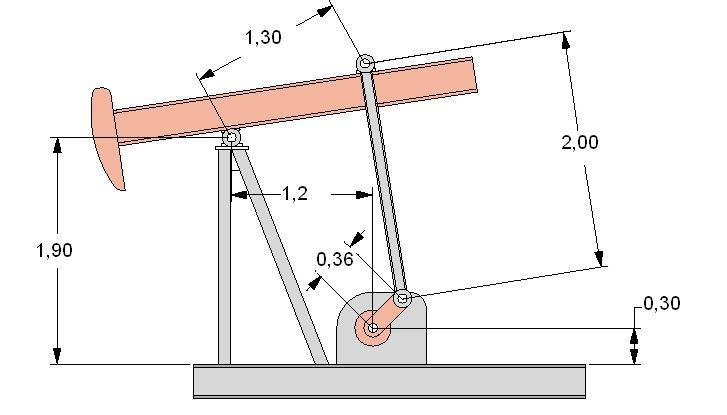
\includegraphics[width=0.9\textwidth]{images/mec4barras}
    \caption{Exemplo de mecanismo de quatro barras utilizado em bombas de extração de petróleo.}
    \label{fig:mec4barras}
\end{figure}


\section{Conceitos Fundamentais}
\label{sec:conceitos}

Para a cinemática, o entendimento de rotação e translação é fundamental para descrever o comportamento dos corpos.

A rotação, em um sistema 3D é descrita por um vetor de rotação, que é um vetor unitário que indica o eixo de rotação e o sentido da rotação. A magnitude do vetor de rotação é o ângulo de rotação. A rotação de um corpo rígido em torno de um eixo é descrita por um ângulo de rotação e um vetor de rotação.

\begin{figure}[H]
    \centering
    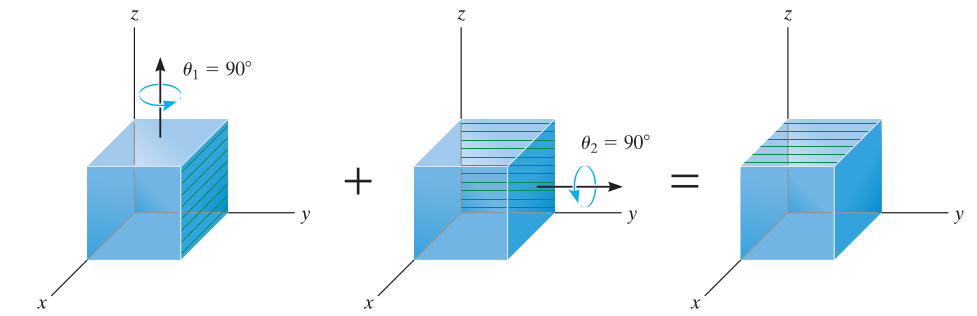
\includegraphics[width=0.9\textwidth]{images/rotacoes}
    \caption{Exemplo de rotação de um corpo rígido em torno de um eixo.}
    \label{fig:rotacao}
\end{figure}

A translação é o movimento de um corpo rígido em que todos os pontos do corpo se movem na mesma direção e sentido. A translação de um corpo rígido é descrita por um vetor de translação, que é um vetor que indica a direção e o sentido do movimento. A magnitude do vetor de translação é a distância percorrida pelo corpo.
    \input{docs/relatorio/2_objetivos}
    \input{docs/relatorio/desenvolvimento teórico}
    \input{docs/relatorio/metodologia}
    \input{docs/relatorio/considerações}
    \input{docs/relatorio/conclusão}
    \bibliographystyle{abntex2-alf}
    \newpage
    \bibliography{docs/referências}
\end{document}